\documentclass{standalone}
\usepackage{tikzducks}
\definecolor{fskin}{RGB}{161,140,126}%
\definecolor{fbill}{RGB}{238,212,191}%
\definecolor{fhair}{RGB}{89,72,72}%
\begin{document}
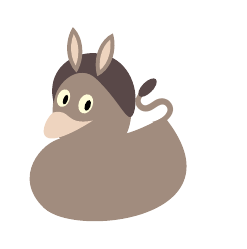
\begin{tikzpicture}
	\duck[body=fskin,bill=fbill,shorthair=fhair,bunny,inear=fbill]
	\node[fskin,rotate=45,scale=3] at (1.7,1.55) {\textsf{s}};
	\fill[fhair,rotate=45] (2.4,0.13) ellipse (0.15 and	0.07);
\end{tikzpicture}
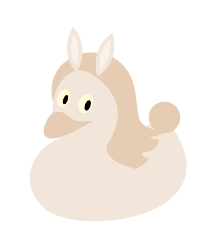
\begin{tikzpicture}
	\duck[body=white!80!brown, bill=white!60!brown, bunny,longhair=white!60!brown]
	\fill[white!60!brown] (tail) circle (0.2);
\end{tikzpicture}
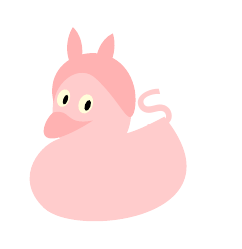
\begin{tikzpicture}
	\duck[body=red!20!white,bill=red!30!white,shorthair=red!30!white,
				bunny=red!30!white,inear=red!30!white]
	\node[red!20!white,rotate=25,scale=3] at (1.7,1.51) {\textsf{s}};
\end{tikzpicture}
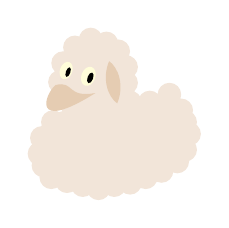
\begin{tikzpicture}
	\duck[body=white!80!brown, bill=white!60!brown, sheep]
\end{tikzpicture}
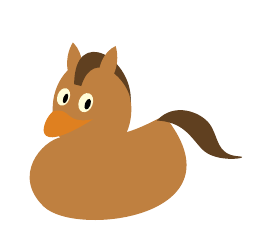
\begin{tikzpicture}
	\begin{scope}[yshift=-6]
		\clip[rotate=-5] (0.68,2.38) ellipse (0.3 and 0.4);
		\fill[brown,rotate=-5](0.28,2.26)ellipse (0.3 and 0.4);
	\end{scope}
	\duck[body=brown,mohican=brown!50!black,horsetail]
	\begin{scope}[yshift=-5,xshift=1]
		\clip[rotate=-5] (0.68,2.38) ellipse (0.3 and 0.4);
		\fill[brown,rotate=-5](1.06,2.2) ellipse (0.3 and 0.4);
	\end{scope}
\end{tikzpicture}
\end{document}